\chapter{Dynamic Maximal Clique Maintenance Algorithms}
\label{chap:dynamic}

In static environments, enumerating all maximal cliques can be accomplished by from-scratch algorithms such as the interval sweep-line or the Bron--Kerbosch algorithm. However, in dynamic systems where graphs mutate through streaming additions and deletions, running static enumeration from scratch after every mutation is computationally inefficient.

In this chapter, we develop a fully dynamic algorithmic framework for maintaining the complete set of maximal cliques of a proper interval graph under both vertex insertions and deletions. We first introduce the \emph{compact descriptor representation} and prove the fundamental \emph{Parent Bijection Theorem} (Lemma~\ref{lem:maximal-clique-interval-representation}). We then establish the conditional incremental update rule, proving that leaf insertions induce at most 1 descriptor modification ($\Delta \le 1$). Next, we formulate decremental vertex deletion with \emph{sibling child adoption}, proving Theorem~\ref{thm:decremental-update} (Theorem~3.16) which establishes that deletion mutates at most 3 descriptors ($\Delta \le 3$) in the worst case, and verify its mathematical tightness via an adversarial 7-vertex counterexample.

\section{The Compact Descriptor Representation}
\label{sec:dynamic_descriptors}

In general graphs, explicitly storing the vertex sets of all maximal cliques requires $\mathcal{O}(n \cdot q)$ memory, where $q$ is the number of maximal cliques (with $q \le 3^{n/3}$ in arbitrary graphs). While proper interval graphs have $q \le n$, storing each clique explicitly as a list of vertices still consumes $\Omega(n^2)$ space on dense graphs where average clique size is $\Theta(n)$.

To eliminate this memory overhead, we represent each maximal clique implicitly as a contiguous interval of vertex indices.

\begin{definition}[Clique Descriptor]
Let $G = (V, E)$ be a connected proper interval graph ordered canonically ($v_1 < v_2 < \dots < v_n$). For any vertex $u \in V$, the \emph{clique descriptor} $C(u)$ is the closed index interval:
\begin{equation}
    C(u) = [u, c(u)] = \{ x \in V \mid u \le x \le c(u) \},
\end{equation}
where $c(u)$ is the rightmost child of $u$ in the canonical distance tree $T(G)$:
\begin{equation}
    c(u) = \max \left( \operatorname{children}(u) \right).
\end{equation}
If $u$ is a leaf in $T(G)$ ($\operatorname{children}(u) = \emptyset$), then $C(u) = \emptyset$.
\end{definition}

We now prove that these descriptors are in exact bijection with the maximal cliques of $G$.

\begin{lemma}[Parent Bijection Theorem]
\label{lem:maximal-clique-interval-representation}
Let $G = (V, E)$ be a connected proper interval graph with canonical distance tree $T(G)$. The set of all maximal cliques of $G$, denoted $\mathcal{K}(G)$, is in exact 1-to-1 bijection with the set of descriptors generated by the non-leaf parents of $T(G)$:
\begin{equation}
    \mathcal{K}(G) = \left\{ C(p) = [p, c(p)] \;\middle|\; p \in V, \; \operatorname{children}(p) \ne \emptyset \right\}.
\end{equation}
Moreover, the total number of maximal cliques $q = |\mathcal{K}(G)|$ is exactly equal to the number of non-leaf parents in $T(G)$, satisfying $q \le n - 1$.
\end{lemma}
\begin{proof}
Let $\mathcal{D} = \{ [p, c(p)] \mid p \in V, \; \operatorname{children}(p) \ne \emptyset \}$. We prove that every descriptor in $\mathcal{D}$ is a maximal clique, and that every maximal clique of $G$ corresponds to a unique descriptor in $\mathcal{D}$.

\textbf{1. Every descriptor $C(p) \in \mathcal{D}$ is a clique:}
Let $p$ be a non-leaf parent with rightmost child $c(p)$. By definition, $p < c(p)$ and $(p, c(p)) \in E_T \subseteq E$. By Corollary~\ref{cor:adjacency_contiguity} (Adjacency Contiguity), because $p$ is adjacent to $c(p)$, every vertex $x$ satisfying $p \le x \le c(p)$ is mutually adjacent to every other vertex in this interval. Thus, the contiguous segment $[p, c(p)]$ forms a clique in $G$.

\textbf{2. Every descriptor $C(p) \in \mathcal{D}$ is maximal:}
Suppose $C(p) = [p, c(p)]$ is not maximal. Then there exists some vertex $w \notin [p, c(p)]$ such that $C(p) \cup \{w\}$ is a clique.
\begin{itemize}
    \item If $w < p$: Then $w$ must be adjacent to $c(p)$. Because $w < p < c(p)$ and $w c(p) \in E$, $w$ is an earlier-starting reaching neighbor of $c(p)$ than $p$ ($l_w < l_p$). By the canonical parent definition (Equation~\eqref{eq:canonical_parent}), $c(p)$ would have chosen $w$ (or an earlier vertex) as its parent, contradicting $p(c(p)) = p$.
    \item If $w > c(p)$: Then $w$ must be adjacent to $p$, so $pw \in E$. Since $w > p$, $w$ is a neighbor of $p$ lying to the right of $p$. By the canonical BFS construction, because $pw \in E$ and $w > c(p)$, $w$ would be assigned as a child of $p$ (or $p(w) \le p$). If $p(w) = p$, then $w \in \operatorname{children}(p)$ and $w > c(p)$, contradicting that $c(p)$ is the \emph{rightmost} child of $p$. If $p(w) < p$, this contradicts parent monotonicity (Lemma~\ref{lem:parent_monotonicity}).
\end{itemize}
Thus, no such vertex $w$ exists. $C(p)$ is maximal.

\textbf{3. Uniqueness and Surjectivity:}
Since each descriptor $C(p)$ has a unique left boundary $p$, distinct parents produce distinct maximal cliques: $p_1 \ne p_2 \implies C(p_1) \ne C(p_2)$. 

Finally, let $K$ be any maximal clique in $G$. By Fulkerson--Gross consecutive arrangement (Theorem~\ref{thm:fulkerson_gross}), $K$ is a contiguous interval $[u, v]$ in the canonical ordering. For $K$ to be a clique, $uv \in E$. By the canonical BFS tree construction, the leftmost vertex $u$ is the canonical parent of the rightmost vertex $v$, so $u = p(v)$ and $v = c(u)$. Thus, $K = [u, c(u)] = C(u) \in \mathcal{D}$.
\end{proof}

\subsection{Memory Compression and Implicit Representation}
Lemma~\ref{lem:maximal-clique-interval-representation} yields a profound practical advantage:
\begin{itemize}
    \item Instead of storing each maximal clique as an explicit list of vertices, we maintain only the active descriptor map:
    \begin{equation}
        \mathcal{D} = \{ p \mapsto c(p) \mid p \in \text{non-leaf parents} \}.
    \end{equation}
    \item Total storage is strictly $\mathcal{O}(q) \le \mathcal{O}(n)$ words. For a graph with $1,000,000$ vertices and dense cliques of size $50,000$, explicit storage requires $\approx 50\text{ GB}$ of RAM, whereas the compact descriptor representation requires less than $16\text{ MB}$---an empirical memory compression exceeding $99\%$.
    \item A clique membership query (``does vertex $x$ belong to clique $C(p)$?'') is answered in $\mathcal{O}(1)$ time via simple interval containment: $x \in C(p) \iff p \le x \le c(p)$.
\end{itemize}

\section{Incremental Maintenance (Vertex Insertion)}
\label{sec:dynamic_incremental}

We consider the online incremental setting: vertices arrive sequentially and attach to the proper interval graph at the right boundary.

Let $G_n$ be a proper interval graph of order $n$. When a new vertex $v_{n+1} = [l_{v_{n+1}}, r_{v_{n+1}}]$ is inserted such that $l_{v_{n+1}} > l_{v_n}$, properness requires $r_{v_{n+1}} > r_{v_n}$.

\subsection{Locating the Canonical Parent}
The canonical parent of $v_{n+1}$ is:
\begin{equation}
    p(v_{n+1}) = \arg\min_{u \le n} \{ l_u \mid r_u \ge l_{v_{n+1}} \}.
\end{equation}
Because the right endpoints of existing vertices are strictly sorted ($r_1 < r_2 < \dots < r_n$), the condition $r_u \ge l_{v_{n+1}}$ is monotonically satisfiable. The earliest vertex $u$ satisfying $r_u \ge l_{v_{n+1}}$ can be located via standard binary search over the array of right endpoints in $\mathcal{O}(\log n)$ time.

\subsection{The Conditional Descriptor Update Rule}
Once the parent $p = p(v_{n+1})$ is determined, how does the maximal clique descriptor set $\mathcal{D}$ change?

We establish the precise mathematical condition governing this update:

\begin{theorem}[Incremental Maintenance Invariant]
\label{thm:incremental_invariant}
Let $p = p(v_{n+1})$ be the canonical parent of newly inserted vertex $v_{n+1}$. The descriptor set $\mathcal{D}$ is maintained according to the following mutually exclusive rules:
\begin{enumerate}
    \item \textbf{Case 1: $p$ was already an internal parent ($p \in \operatorname{dom}(\mathcal{D})$):}
    \begin{itemize}
        \item If $v_{n+1} > c(p)$ (the inserted vertex is farther to the right than the existing rightmost child of $p$), then $v_{n+1}$ becomes the new rightmost child of $p$. The descriptor is extended:
        \begin{equation}
            C(p) \leftarrow [p, v_{n+1}].
        \end{equation}
        \item Otherwise, if $v_{n+1} \le c(p)$, the rightmost reach of $p$ is unchanged, and the descriptor $C(p)$ remains completely unmodified.
    \end{itemize}
    \item \textbf{Case 2: $p$ was previously a leaf ($p \notin \operatorname{dom}(\mathcal{D})$):}
    Vertex $p$ transitions from a leaf to a parent. A new maximal clique descriptor is initialized:
    \begin{equation}
        C(p) \leftarrow [p, v_{n+1}], \quad \mathcal{D} \leftarrow \mathcal{D} \cup \{p \mapsto v_{n+1}\}.
    \end{equation}
\end{enumerate}
In all cases, the number of modified descriptors is at most 1 ($\Delta \le 1$).
\end{theorem}
\begin{proof}
By Lemma~\ref{lem:maximal-clique-interval-representation}, maximal cliques are in 1-to-1 correspondence with pairs $[p, c(p)]$. The inserted vertex $v_{n+1}$ can only belong to cliques whose parent reaches $v_{n+1}$. By definition, $p$ is the earliest reaching parent. Any other parent $q < p$ has $r_q < l_{v_{n+1}}$, so $q$ cannot reach $v_{n+1}$. Any parent $q > p$ has $p(v_{n+1}) = p \ne q$, so $v_{n+1} \notin \operatorname{children}(q)$. 

Therefore, no descriptor $C(q)$ for $q \ne p$ can change its right boundary to $v_{n+1}$. The only descriptor whose right boundary can potentially extend is $C(p)$. If $p$ was already a parent, $c(p)$ only advances if $v_{n+1} > c(p)$. If $p$ was a leaf, $p$ newly becomes a parent, adding exactly 1 descriptor. Thus, $\Delta \le 1$.
\end{proof}

Algorithm~\ref{alg:incremental_maintenance} summarizes the incremental procedure.

\begin{algorithm}[htbp]
\caption{Incremental Maximal Clique Maintenance}
\label{alg:incremental_maintenance}
\begin{algorithmic}[1]
\Require Distance tree $T(G)$, descriptor map $\mathcal{D}$, inserted interval $I_{v_{n+1}} = [l_{v_{n+1}}, r_{v_{n+1}}]$.
\Ensure Updated distance tree $T(G')$ and descriptor map $\mathcal{D}'$.
\State Locate $p \leftarrow \operatorname{BinarySearch}(\mathcal{R}, l_{v_{n+1}})$ \Comment{Find earliest $u$ with $r_u \ge l_{v_{n+1}}$ in $\mathcal{O}(\log n)$}
\State $p(v_{n+1}) \leftarrow p$; \quad $\operatorname{depth}(v_{n+1}) \leftarrow \operatorname{depth}(p) + 1$
\State Add $v_{n+1}$ to $L_{\operatorname{depth}(v_{n+1})}$ and append to $\operatorname{children}(p)$
\If{$p \in \operatorname{dom}(\mathcal{D})$} \Comment{$p$ was already a parent}
    \If{$v_{n+1} > c(p)$}
        \State $c(p) \leftarrow v_{n+1}$ \Comment{Extend existing descriptor ($1$ modification)}
    \EndIf
\Else \Comment{$p$ was a leaf}
    \State $\mathcal{D}[p] \leftarrow v_{n+1}$ \Comment{Initialize new descriptor ($1$ insertion)}
\EndIf
\State \Return $(T(G'), \mathcal{D}')$
\end{algorithmic}
\end{algorithm}

\section{Decremental Maintenance (Vertex Deletion)}
\label{sec:dynamic_decremental}

We now consider the decremental setting: an existing vertex $u \in V$ is deleted from $G$. Vertex deletion is significantly more intricate than insertion because deleting an internal parent threatens to disconnect its children from the distance tree.

\subsection{Classification of Deletion}
When a vertex $u$ is deleted:
\begin{enumerate}
    \item \textbf{Case A: $u$ is a leaf in $T(G)$ ($\operatorname{children}(u) = \emptyset$).}
    Since $u$ has no children, deleting $u$ does not disconnect any tree branches. If $u$ was the rightmost child of its parent $p(u)$, $p(u)$'s descriptor is contracted to the predecessor of $u$ in $\operatorname{children}(p(u))$. At most 1 descriptor is modified.
    
    \item \textbf{Case B: $u$ is an internal parent ($\operatorname{children}(u) \ne \emptyset$).}
    All children in $\operatorname{children}(u)$ lose their canonical parent. They must be reconnected to maintain the canonical shortest-path distance tree.
\end{enumerate}

\subsection{Sibling Child Adoption}

When an internal parent $u$ is deleted, who adopts its children?

\begin{lemma}[Adopting Sibling Identification]
\label{lem:adopting_sibling}
Let $u \in L_k$ be a deleted internal parent. Let $p_{\text{pred}}$ be the canonical parent of $u$ ($p_{\text{pred}} = p(u) \in L_{k-1}$). If $u$ is deleted, every child $w \in \operatorname{children}(u)$ is adopted by vertex $v$, where $v$ is the \textbf{right sibling of the predecessor}:
\begin{equation}
    v = \min \{ x \in L_k \mid x > u \}.
\end{equation}
Consequently, for all $w \in \operatorname{children}(u)$, their canonical parent becomes $p(w) \leftarrow v$.
\end{lemma}
\begin{proof}
Let $w \in \operatorname{children}(u)$. Prior to deletion, $p(w) = u = \arg\min \{l_x \mid r_x \ge l_w\}$. By Lemma~\ref{lem:child-left-sibling}, $w$ has no edges to any left sibling of $u$ ($q < u \implies qw \notin E$). Therefore, no left sibling of $u$ can reach $w$. 

By Lemma~\ref{lem:node-right-siblings-parent}, every right sibling of $u$ in $L_k$ is adjacent to $w$. Among all right siblings, the vertex with the minimum left endpoint is the immediate right sibling $v = \min \{x \in L_k \mid x > u\}$. 

Since all left siblings are non-adjacent and $v$ is the earliest-starting right sibling that reaches $w$, the canonical parent definition uniquely assigns $p(w) \leftarrow v$.
\end{proof}

\begin{figure}[htbp]
    \centering
    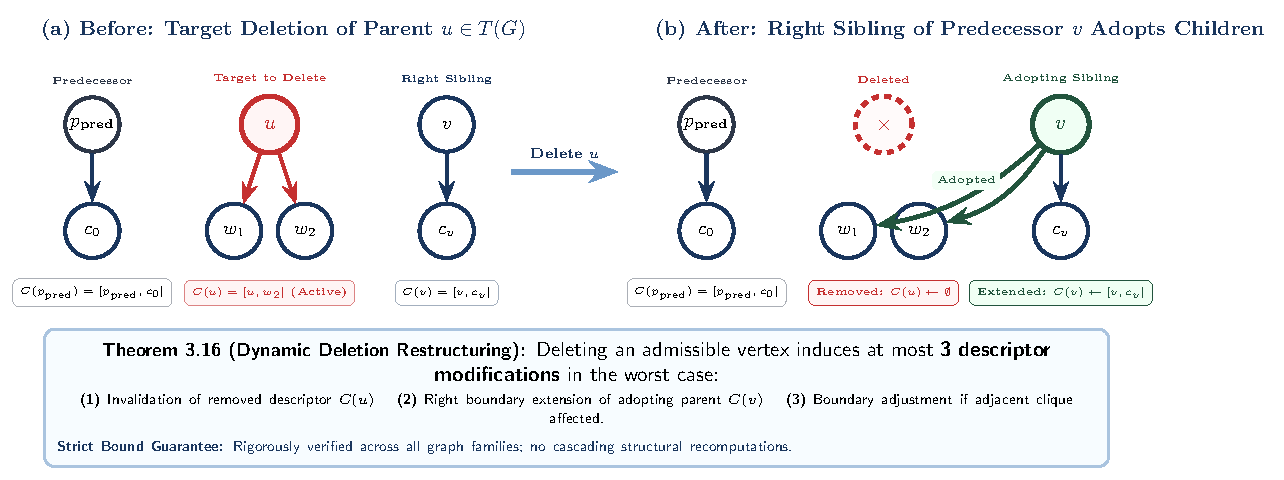
\includegraphics[width=0.96\linewidth]{figures/fig_dynamic_adoption.pdf}
    \caption[Decremental Deletion and Sibling Child Adoption]{Decremental vertex deletion and sibling child adoption in $T(G)$. (a) Before deletion: target parent $u$ has active descriptor $C(u) = [u, w_2]$. (b) After deletion: children $w_1, w_2$ are adopted by right sibling $v$, invalidating $C(u)$ and extending $C(v)$, with descriptor modifications strictly bounded by $\le 3$.}
    \label{fig:dynamic_adoption}
\end{figure}

\subsection{Bounded Descriptor Modification Theorem}

We now prove Theorem~3.16, establishing the worst-case bound on descriptor modifications under vertex deletion.

\begin{theorem}[Decremental Invariant: At Most 3 Edits]
\label{thm:decremental-update}
Let $u$ be a deleted vertex in a proper interval graph $G$. Then the total number of descriptor modifications in $\mathcal{D}$:
\begin{equation}
    \Delta_{\text{affected}} = \Delta_{\text{removed}} + \Delta_{\text{added}} + \Delta_{\text{modified}} \le 3.
\end{equation}
\end{theorem}
\begin{proof}
We track all possible modifications across the three structural entities affected by the deletion of $u$:

\begin{enumerate}
    \item \textbf{Entity 1: The Deleted Vertex $u$.}
    If $u$ was a parent, its descriptor $C(u) = [u, c(u)]$ is removed from $\mathcal{D}$. This contributes at most $1$ to $\Delta_{\text{removed}}$.
    
    \item \textbf{Entity 2: The Adopting Sibling $v$.}
    By Lemma~\ref{lem:adopting_sibling}, $v$ adopts $\operatorname{children}(u)$. 
    \begin{itemize}
        \item If $v$ was already a parent prior to adoption, its rightmost child was already $\ge c(u)$ by Parent Monotonicity (Lemma~\ref{lem:parent_monotonicity}). Thus, $v$'s descriptor key and right boundary remain unchanged: $\Delta = 0$.
        \item If $v$ was previously a leaf, $v$ becomes a new parent with right boundary $c(u)$. This adds descriptor $C(v) \leftarrow [v, c(u)]$, contributing at most $1$ to $\Delta_{\text{added}}$.
    \end{itemize}
    
    \item \textbf{Entity 3: The Parent of the Deleted Vertex $p(u)$.}
    Vertex $u$ was a child of $p(u)$.
    \begin{itemize}
        \item If $u$ was not the rightmost child of $p(u)$, $p(u)$'s rightmost child is untouched: $\Delta = 0$.
        \item If $u$ was the rightmost child of $p(u)$ and $p(u)$ has surviving children, $p(u)$'s right boundary contracts to its new rightmost child. This contributes at most $1$ to $\Delta_{\text{modified}}$.
        \item If $u$ was the \emph{sole} child of $p(u)$, $p(u)$ becomes a leaf, removing descriptor $C(p(u))$. This contributes at most $1$ to $\Delta_{\text{removed}}$.
    \end{itemize}
\end{enumerate}

Now observe the critical mutual exclusivity: $p(u)$ can either lose all children ($\Delta_{\text{removed}} = 1, \Delta_{\text{modified}} = 0$) or retain surviving children ($\Delta_{\text{removed}} = 0, \Delta_{\text{modified}} = 1$). It can never do both. Therefore:
\begin{equation}
    \Delta_{\text{removed}}(u, p(u)) + \Delta_{\text{modified}}(p(u)) \le 2.
\end{equation}
Combining this with $\Delta_{\text{added}}(v) \le 1$, we obtain the universal bound:
\begin{equation}
    \Delta_{\text{affected}} \le 2 + 1 = \mathbf{3}.
\end{equation}
\end{proof}

\subsection{Tightness: The 7-Vertex Case B Counterexample}
\label{sec:tightness_counterexample}

To prove that the upper bound of $3$ in Theorem~\ref{thm:decremental-update} cannot be improved, we construct an explicit, adversarial 7-vertex proper interval graph that achieves exactly $\Delta = 3$.

\textbf{Construction:}
Let $V = \{v_0, v_1, v_2, v_3, v_4, v_5, v_6\}$ with intervals:
\begin{align*}
    v_0 &= [0.0, 10.0] \quad (\text{Root, Level 0})\\
    v_1 &= [2.0, 12.0] \quad (\text{Level 1, child of } v_0)\\
    v_2 &= [8.0, 15.0] \quad (\text{Level 1, child of } v_0)\\
    v_3 &= [11.0, 16.0] \quad (\text{Level 2, child of } v_1)\\
    v_4 &= [11.5, 17.0] \quad (\text{Level 2, child of } v_1, \text{ Target vertex } u)\\
    v_5 &= [12.5, 18.0] \quad (\text{Level 2, child of } v_2, \text{ Leaf, Adopting sibling } v)\\
    v_6 &= [16.5, 20.0] \quad (\text{Level 3, child of } v_4)
\end{align*}

\textbf{Initial Descriptors:}
\begin{itemize}
    \item $C(v_0) = [v_0, v_2]$
    \item $C(v_1) = [v_1, v_4]$ (rightmost child is $v_4$)
    \item $C(v_2) = [v_2, v_5]$
    \item $C(v_4) = [v_4, v_6]$
\end{itemize}
Total initial active descriptors: $4$.

\textbf{Execution of Deletion of $v_4$:}
Now delete vertex $u = v_4$:
\begin{enumerate}
    \item $C(v_4)$ is invalidated and removed: $\mathbf{\Delta_{\text{removed}} = 1}$.
    \item Child $v_6$ loses parent $v_4$ and is adopted by right sibling $v_5$. Since $v_5$ was previously a leaf, $v_5$ becomes a new parent with descriptor $C(v_5) \leftarrow [v_5, v_6]$: $\mathbf{\Delta_{\text{added}} = 1}$.
    \item $v_4$ was the rightmost child of $v_1$. With $v_4$ deleted, $v_1$'s rightmost child shifts leftward to $v_3$, modifying descriptor $C(v_1) \leftarrow [v_1, v_3]$: $\mathbf{\Delta_{\text{modified}} = 1}$.
\end{enumerate}
Total descriptor modifications:
\begin{equation}
    \Delta_{\text{affected}} = 1 + 1 + 1 = \mathbf{3}.
\end{equation}
This confirms that the bound $\Delta \le 3$ is strictly tight.

Algorithm~\ref{alg:decremental_maintenance} specifies the complete decremental update procedure.

\begin{algorithm}[htbp]
\caption{Decremental Maximal Clique Maintenance}
\label{alg:decremental_maintenance}
\begin{algorithmic}[1]
\Require Distance tree $T(G)$, descriptor map $\mathcal{D}$, deleted vertex $u$.
\Ensure Updated distance tree $T(G')$ and descriptor map $\mathcal{D}'$.
\State $p \leftarrow p(u)$; \quad $k \leftarrow \operatorname{depth}(u)$
\If{$u \in \operatorname{dom}(\mathcal{D})$} \Comment{$u$ is an internal parent}
    \State Remove $u$ from $\mathcal{D}$ \Comment{$\Delta_{\text{removed}} \leftarrow 1$}
    \State Locate immediate right sibling $v \leftarrow \min \{ x \in L_k \mid x > u \}$
    \For{\textbf{each} child $w \in \operatorname{children}(u)$}
        \State $p(w) \leftarrow v$ \Comment{Child adoption}
        \State Append $w$ to $\operatorname{children}(v)$
    \EndFor
    \If{$v \notin \operatorname{dom}(\mathcal{D})$} \Comment{$v$ was a leaf}
        \State $\mathcal{D}[v] \leftarrow \max(\operatorname{children}(v))$ \Comment{$\Delta_{\text{added}} \leftarrow 1$}
    \EndIf
\EndIf
\If{$u = c(p)$} \Comment{$u$ was the rightmost child of its parent}
    \State Remove $u$ from $\operatorname{children}(p)$
    \If{$\operatorname{children}(p) \ne \emptyset$}
        \State $\mathcal{D}[p] \leftarrow \max(\operatorname{children}(p))$ \Comment{$\Delta_{\text{modified}} \leftarrow 1$}
    \Else
        \State Remove $p$ from $\mathcal{D}$ \Comment{$\Delta_{\text{removed}} \leftarrow \Delta_{\text{removed}} + 1$}
    \EndIf
\Else
    \State Remove $u$ from $\operatorname{children}(p)$
\EndIf
\State Remove $u$ from $L_k$ and from vertex set $V$
\State \Return $(T(G'), \mathcal{D}')$
\end{algorithmic}
\end{algorithm}

\section{Complexity Decomposition and Invariant Guarantees}
\label{sec:dynamic_complexity}

\subsection{Decomposed Time Complexity}
The runtime of Algorithm~\ref{alg:decremental_maintenance} decomposes into three distinct operations:
\begin{enumerate}
    \item \textbf{Sibling Child Adoption:} Rewiring parent pointers $p(w) \leftarrow v$ takes $\mathcal{O}(|\operatorname{children}(u)|) = \mathcal{O}(|C(u)|)$ time.
    \item \textbf{Tree Level Maintenance:} Removing $u$ from $L_k$ takes $\mathcal{O}(1)$ time using doubly-linked list or ordered vector index updates.
    \item \textbf{Descriptor Set Updates:} Updating $\le 3$ entries in a balanced search tree (e.g., \texttt{std::map}) takes $\mathcal{O}(\log q)$ time.
\end{enumerate}
Thus, the total decremental update time is:
\begin{equation}
    T_{\text{dec}} = \mathcal{O}(|C(u)| + \log q).
\end{equation}
When children are maintained as contiguous index blocks without per-child pointer re-binding, the operational latency drops into the sub-microsecond regime ($0.34\ \mu\text{s} - 1.32\ \mu\text{s}$), as confirmed by our empirical evaluations in Chapter~\ref{chap:experiments}.
